\chapter{Related Work}
\setcounter{section}{0}

\section{Background}

\section{Indico}


\subsection{Events}

\begin{figure}[H]
    \centering
    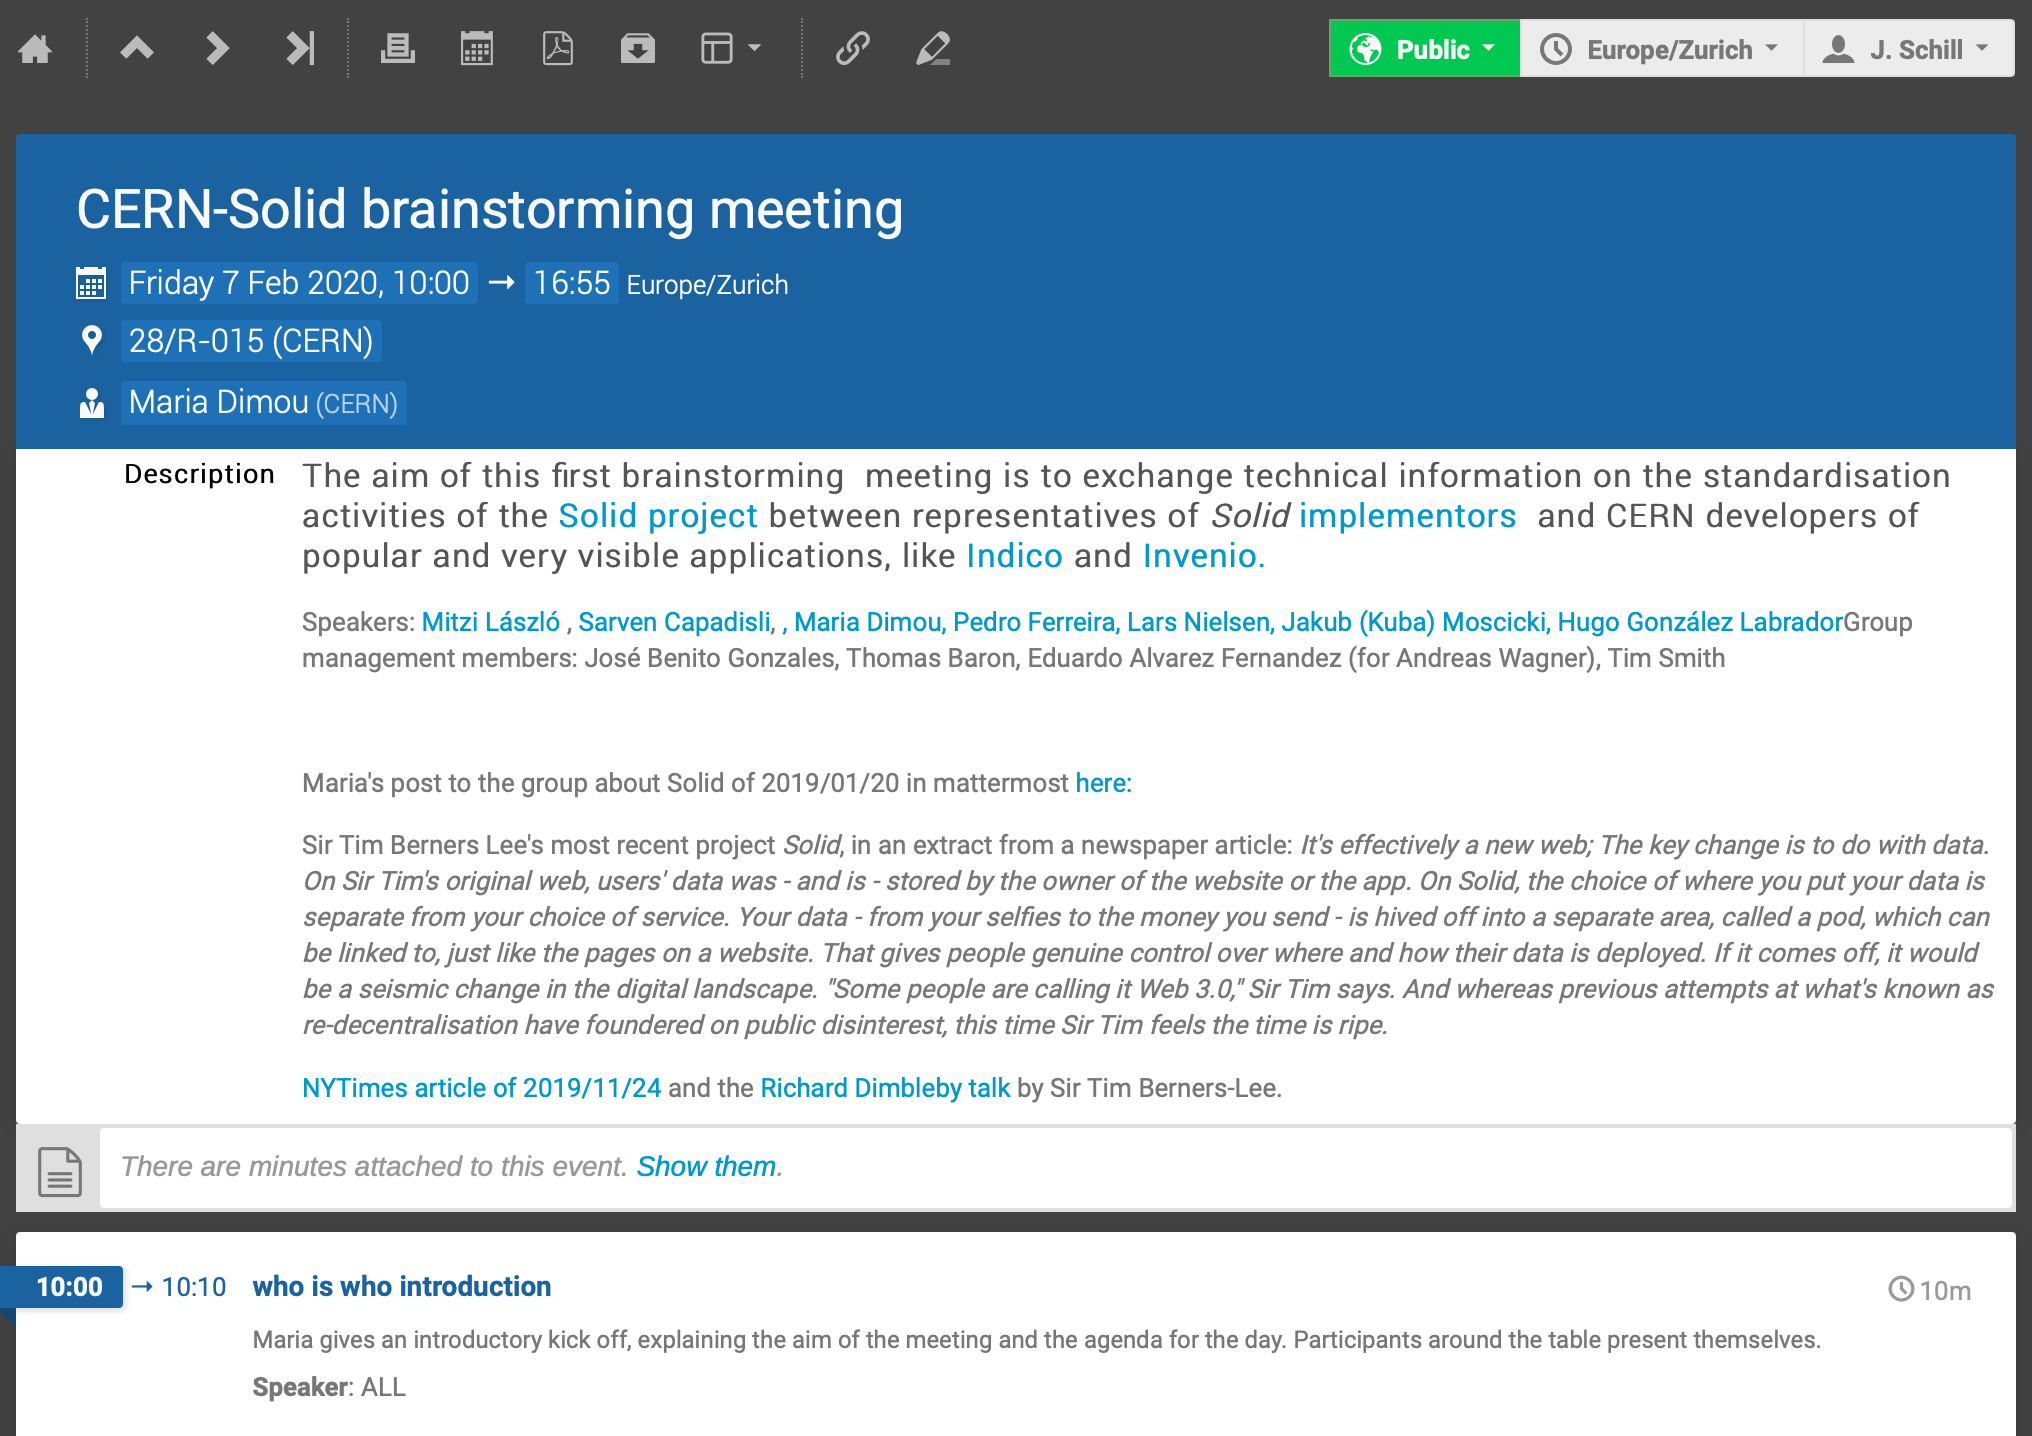
\includegraphics[width=0.6\textwidth]{thesis/latex/assets/indico-event-interface.png}
    \caption{User interface of an Indico event.}
    \label{fig:indico-event-interface}
\end{figure} 

\subsection{Storage Mechanisms}

\subsubsection{EventSettingsProxy}

\subsection{Conference Registration}

\section{Solid}

A prior introduction to Solid was given as part of a previous \textit{research project} \cite{cern-solid-investigation-spec} in preparation to this thesis. In the \textit{research project} the Solid specification was among other things summarized and analyzed. This section will reiterate and study the to the subsequent experiment relevant parts further.

\subsection{Authentication With Solid}

In the Solid ecosystem agents identify themselves with their WebID and proof their ownership through the \gls{solidoidc} protocol, which is a flavor of \gls{oidc}. For further explanation and flow diagrams through the authentication process see either the work done in the previous report \cite{cern-solid-investigation-spec} or the \gls{solidoidc} specification itself \cite{solid-ecosystem-oidc}.

To help with the complex authentication flow of \gls{solidoidc} a few libraries have been developed by different actors. Two libraries relevant for this project exist, their relevancy is discussed in chapter \ref{chapter:investigation} under the section \ref{subsubsection:design}.

\begin{table}[h!]
    \centering
    \begin{tabular}{| l | l | l |} 
     \hline
     Name & Solid Auth Fetcher & solid-client-authn \\
     \hline
     Repository URL & \url{github.com/solid/solid-auth-fetcher} & \url{github.com/inrupt/solid-client-authn-js} \\
     \hline
     Language & \gls{ts} & \gls{ts} \\
     \hline
     Maintainer & Solid Community & Inrupt \\
     \hline
     Last updated & 2021/03/05 & 2021/05/12 \\
     \hline
    \end{tabular}
    \vspace{0.75cm}
    \caption{Two Solid authentication libraries.}
    \label{table:0}
\end{table}

Solid Auth Fetcher is a fork of the \texttt{solid-client-authn} developed by Inrupt, but has not seen much development in recent time. With the quickly evolving Solid ecosystem it is important to have working and up-to-date libraries to be able to build applications in this ecosystem. Both libraries do not differ in their core functionality and both support authenticating with the latest Solid servers and thus the choice is not as important. Still, the frequency of commits in Inrupt's repository seem to indicate a more active development and thus a more reliable source when problems arise. This way one does not rely on the support from open-source developers, which is per se not a bad thing.

For this simple reason all programming where Solid authentication was needed was enabled through Inrupt's \texttt{solid-client-authn}.

\subsection{Reading and Writing Linked Data}

Data in Solid is stored as Linked Data \cite{Malhotra:15:LDP}. \gls{rdf} is a framework for representing information in form of Linked Data in the Web \cite{Cyganiak:14:RCA}. The default file format so far implemented by the existing Solid servers is \textit{Turtle} \cite{Prud:hommeaux:14:RT}.

The graph-based data model from using \gls{rdf} also requires additional computing as it is not natively supported with helper functions in \gls{js}, such as \gls{json}. The benefit of using \gls{json} in \gls{js} is that a \gls{json} object is automatically parsed as an object and can be operated on by using the dot notation to access attributes of the \gls{json} data structure. This is not the case for a into the program loaded Turtle resource.

Fortunately, existing libraries come to rescue allowing such operations on the \gls{rdf}-based data type. Again Inrupt and the Solid Community offer solutions. Again, Inrupt's solution was chosen for this development as it acts as convenient wrapper to the bare bone Linked Data \gls{api} implemented in \texttt{rdflib.js} \cite{rdflib-js}. Even though working with \gls{rdf} can be easily done with just using \texttt{rdflib.js}, Inrupt's libraries tie nicely together and allow for instance an seamless passing of an authenticated session to its client library to enable authenticated requests to protected resources.

As mentioned before and looked at in detail in \cite{cern-solid-investigation-spec} the Turtle format is a graph data structure build up with triplets. A triplet statement in its simplest form a sequence of (subject, predicate, object) terms \cite{Prud:hommeaux:14:RT}. 

Inrupt decided to call this construct a \texttt{Thing}, which is a data entity associated with a set of data or properties of this \texttt{Thing} \cite{thing}. A \texttt{SolidDataset} is a set of things \cite{inrupt-dataset}.

The following code listing shows how the helper methods can be used to extract data from a Turtle file loaded by a request to the WebID profile document \gls{uri}.

\begin{lstlisting}[language=Other,columns=fullflexible, caption={TODO: Label caption}, label={lst:2}]
// 1
const myDataset = await getSolidDataset(
  "https://janschill.net/profile/card"
);
// 2
const myProfile = getThing(
  myDataset,
  "https://janschill.net/profile/card#me"
);
// 3
const fn = getStringNoLocale(myProfile, VCARD.fn);


\end{lstlisting}

\begin{enumerate}
    \item Notice here the WebID profile document \gls{uri} is being loaded, which refers to the document describing the agent behind the WebID \gls{uri}
    \item Now the actual triplet statement containing information behind this specific agent is mapped to the \texttt{myProfile} variable
    \item Every subject and predicate is a \gls{uri} as
\end{enumerate}

\subsection{Authorization Through WAC}

\subsection{Application Launcher}
